\pgfplotsset{compat = newest}
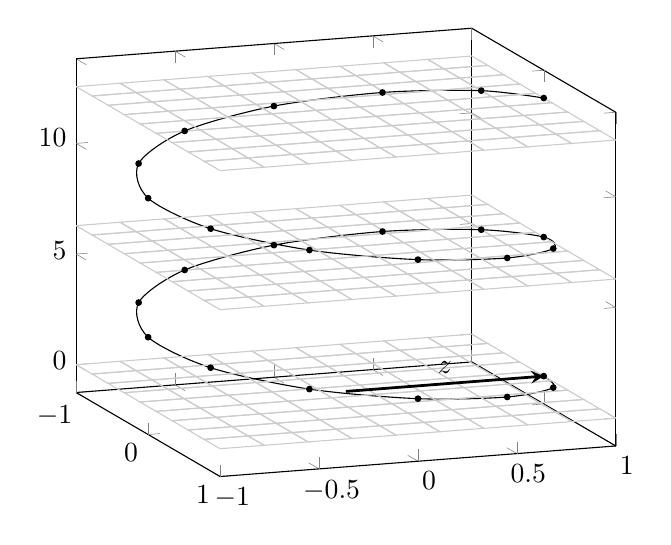
\begin{tikzpicture}
\begin{axis}[view={70}{15}]
    \addplot3+ [mark options={scale=0.5,fill=black,draw=black,},smooth,black,domain=0:4*pi,samples y=0] ({sin(deg(x))},{cos(deg(x))},{x});
    \addplot3+ [thin,no markers,mesh,draw=gray!40,domain=-1:1,samples=10] {2*pi};
    \addplot3+ [thin,no markers,mesh,draw=gray!40,domain=-1:1,samples=10] {0};
    \addplot3+ [thin,no markers,mesh,draw=gray!40,domain=-1:1,samples=10] {4*pi};
    \draw [line width=1pt,black,-stealth](0,0,0)--(0,1,0) node[midway, above]{$z$};
\end{axis}
\end{tikzpicture}
\caption{Representación de un numero $z=1[\cos{(\phi)}+j\sen{(\phi)}]$ siendo $\phi$ una variable correspondiente al eje $z$.}
